\documentclass[12pt,a4paper]{article}
\usepackage{indentfirst}
\usepackage[utf8x]{inputenc}
\usepackage{ucs}
\usepackage[MeX]{polski}
\usepackage{fancyhdr}
\usepackage{amsmath}
\usepackage{amsfonts}
\usepackage{amssymb}
\usepackage{subfig}
%\usepackage{supertabular}
\usepackage{array}
\usepackage{tabularx}
\usepackage{hhline}
\usepackage{tabulary, booktabs}
\usepackage{float}
\usepackage{lscape}
\usepackage[table]{xcolor}
\pagestyle{fancy}
\usepackage{graphicx}
\usepackage{multirow}
\usepackage[final]{pdfpages}
\newenvironment{bottompar}{\par\vspace*{\fill}}{\clearpage}
 
\begin{document}
\clearpage
\thispagestyle{empty}
 
\begin{figure}[H]
\centering

\includegraphics[scale=1.3]{logo.png}
\end{figure}
 
\vspace{16pt}
 
\begin{center}
\textbf{\huge Bazy Danych (Projekt)}
 
\vspace{30pt}
 
\textbf{\LARGE Analiza danych pogodowych}
 
 
\vspace{22pt}
 
\LARGE Opis projektu
 
\end{center}
 
\vspace{20pt}
 
\begin{flushleft}
Autorzy: Dymitr Choroszczak 218627, Krzysztof Dąbek 218549\\
Kurs: Bazy danych (projekt)\\
Temat: Analiza danych\\
Prowadzący: dr hab. inż. Grzegorz Mzyk, prof. PWr\\
Termin zajęć: piątek 9:15\\
\end{flushleft} 
 
\newpage
 
\tableofcontents
 
\newpage
 
\section{Opis projektu}
 
\subsection{Koncept projektu}
\normalsize
Projekt jest realizowany w ramach kursu Bazy Danych na specjalności Robotyka (ARR), na kierunku Automatyka i Robotyka (AiR), na wydziale Elektroniki (EKA), na Politechnice Wrocławskiej.\par
Celem projektu jest stworzenie bazy danych przechowującej informacje pogodowe z różnych stacji, pobierane z serwera oraz zaimplementowanie metod analizy danych i wizualizacji wyników.\par
Dane do analizy zostaną pobrane z serwera ogimet.com dla wielu stacji pogodowych w Polsce i zapisane w tabelach. Dane będą pobierane z witryny za pomocą skryptu napisanego w języku Python, uruchamianego cyklicznie przez skrypt bazy.\par
Zostaną stworzone tabele z danymi, przechowujące podstawowe informacje o wszystkich aktualizowanych stacjach oraz pomiary meteo w pobliżu danej stacji z kolejnych dni.\par
Wynikiem analizy danych są wykresy zależności różnych czynników pogodowych od siebie, wykresy porównawcze dla różnych stacji pogodowych, autokorelacja i korelacja wzajemna pomiarów, automatycznie generowany komentarz dotyczący warunków w pobliżu danej stacji oraz komentarz analityka.
\newpage
\subsection{Wymagania}
\subsubsection{Wymagania funkcjonalne}
\begin{enumerate}
\item Codzienna aktualizacja danych pogodowych
\item Ręczna aktualizacja danych pogodowych
\item Generowanie wykresów analitycznych
\item Generowanie automatycznej analizy
\item Wprowadzanie, zmiana komentarza analityka
\item Wyświetlanie informacji o stacjach pogodowych
\item Wyświetlanie danych pogodowych stacji
\item Wyświetlanie wyników analizy pogody
\item Dodawanie, usuwanie, zmiana stacji pogodowych
\item Logowanie administratorów i analityków
\item Przeprowadzanie wszystkich powyższych operacji tylko w zakresie uprawnień klienta
\end{enumerate}
\subsubsection{Wymagania niefunkcjonalne}
\begin{enumerate}
\item Odporność na utratę danych
\item Bezpieczeństwo danych administratorów i analityków
\item Wydajność
\item Komunikacja z serwerem danych pogodowych
\end{enumerate}

\newpage
\subsection{Tabele i zależności}

\begin{figure}[!htb]
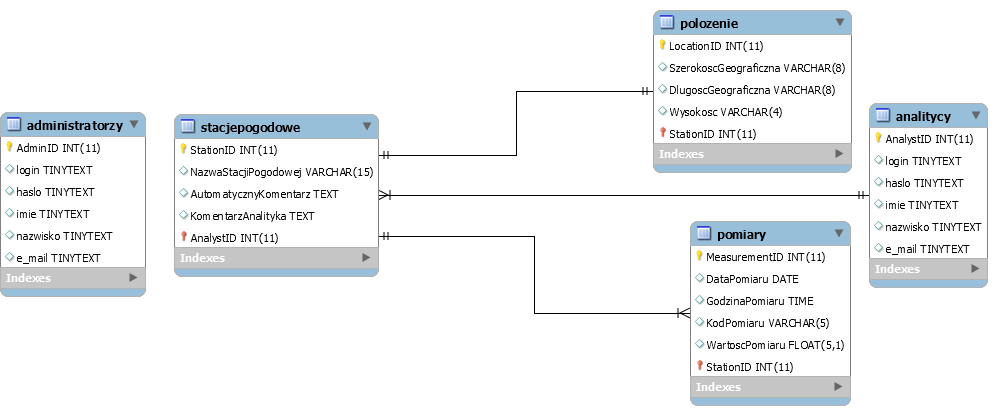
\includegraphics[width=\textwidth]{./figures/diagram_zwiazkow.png}
\caption{Diagram zależności EER}
\end{figure}

\begin{footnotesize}
\begin{itemize}
\item Stacje pogodowe (StationID)
    \begin{itemize}
    \item Nazwa Stacji Pogodowej
    \item Automatyczny komentarz (Wynik analizy danych)
    \item Komentarz analityka (Wynik analizy danych)
    \item Analityk (AnalystID)
    \end{itemize}
\item Pomiary (MeasurementID)
    \begin{itemize}
    \item DataPomiaru
    \item GodzinaPomiaru
    \item KodPomiaru
    \item WartośćPomiaru
    \item Stacja Pogodowa (StationID)
    \end{itemize}
\item Położenie (LocalizationID)
	\begin{itemize}
	\item Szerokość geograficzna
    \item Długość geograficzna
    \item Wysokość (m n.p.m.)
    \item Stacja Pogodowa (StationID)
	\end{itemize}
\item Administratorzy (AdminID)
    \begin{itemize}
    \item Login
    \item Hasło
    \item Imię
    \item Nazwisko
    \item e-mail
    \end{itemize}
\item Analitycy (AnalystID)
    \begin{itemize}
    \item Login
    \item Hasło
    \item Imię
    \item Nazwisko
    \item e-mail
    \end{itemize}
\end{itemize}
\end{footnotesize}
Kod Pomiaru jest tablicą maksymalnie 4 znaków jednoznacznie identyfikujących typ wielkości fizycznej przechowywanej w tym rzędzie:
\begin{itemize}
\item TMAX - Maksymalna dzienna/godzinowa temperatura powietrza ($^\circ C$)
\item TMIN - Minimalna dzienna/godzinowa temperatura powietrza ($^\circ C$)
\item TMID - Średnia dzienna/godzinowa temperatura powietrza ($^\circ C$)
\item HAVG - Średnia wilgotność powietrza (\%)
\item WINT - Średnia prędkość wiatru (km/h)
\item WGUS - Prędkość wiatru w porywach (km/h)
\item PRES - Ciśnienie (hPa)
\item PREC - Opady ogólnie (deszcz, śnieg) (mm)
\item TCLD - Zachmurzenie całkowite
\item LCLD - Zachmurzenie w dolnych partiach
\item SUNH - Czas słońca (km)
\item SVIS - Widoczność (km)
\end{itemize}
\newpage
\subsection{Lista funkcjonalności}
%tabelka z rolami uzytkownikow
\begin{table}[!htb]
\centering
\caption{Poziomy kompetencji klientów} 
  \resizebox{0.9\textwidth}{!}{\begin{tabular}{ | c | c | c | c |}   
    \hline
    \textbf{Klient }& \textbf{Stacje }& \textbf{Pomiary }& \textbf{Położenie }\\ \hline
    \textbf{Administrator }& owner & owner & owner  \\ \hline
    \textbf{Analityk }& owner & table.readonly & table.readonly \\     \hline
    \textbf{Użytkownik }& table.readonly & table.readonly & table.readonly  \\ \hline
  \end{tabular}}
\end{table}

\begin{table}[!htb]
\centering 
  \resizebox{0.7\textwidth}{!}{\begin{tabular}{ | c | c | c | }   
    \hline
    \textbf{Klient }& \textbf{Administratorzy }& \textbf{Analitycy}\\ \hline    
    \textbf{Administrator }& owner & owner  \\ \hline
    \textbf{Analityk }& - & - \\    \hline
    \textbf{Użytkownik } & - & - \\ \hline
  \end{tabular}}
\end{table}

Rolom przyporządkowanym do poszczególnych użytkowników przyporządkowano następujące przywileje:
\begin{itemize}
\item owner : INSERT, SELECT, UPDATE, CREATE, DELETE
\item table.readonly : SELECT
\end{itemize}

\begin{figure}[!htb]
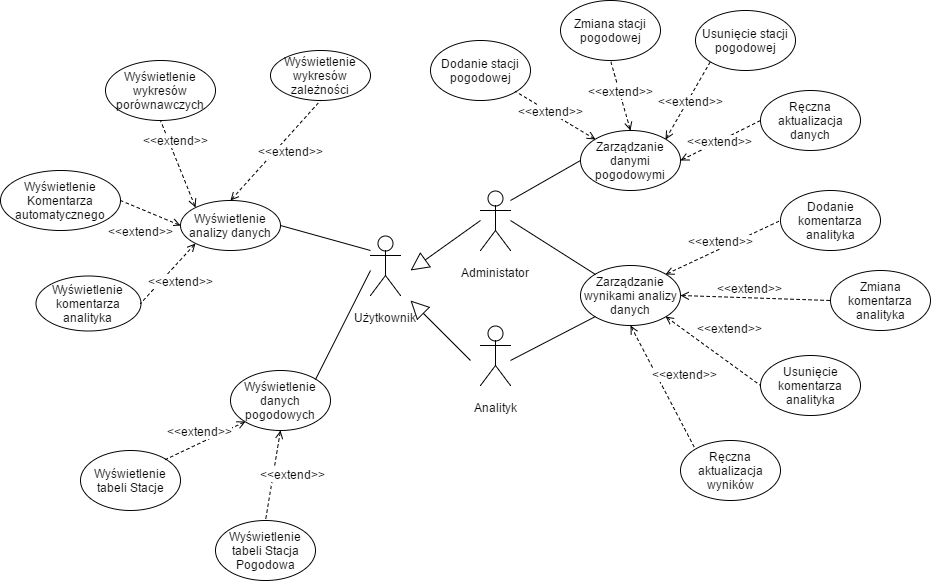
\includegraphics[width=\textwidth]{./figures/DiagramPrzypadkowUzycia.png}
\caption{Diagram przypadków użycia}
\end{figure}
 
 \newpage
\begin{small}
\begin{enumerate}
\item Użytkownik
    \begin{itemize}
    \item Wyświetlenie analizy danych
        \begin{itemize}
        \item Wykresy zależności czynników pogodowych
        \item Wykresy porównawcze warunków między stacjami
        \item Komentarz automatyczny
        \item Komentarz analityka
        \end{itemize}
    \item Wyświetlenie danych pogodowych
        \begin{itemize}
        \item Wyświetlenie tabeli StacjePogodowe
        \item Wyświetlenie tabel Pomiary
        \end{itemize}
    \end{itemize}
\item Administrator (dziedziczy po użytkowniku)
    \begin{itemize}
    \item Zarządzanie danymi pogodowymi
        \begin{itemize}
        \item Dodanie stacji pogodowej
        \item Usunięcie stacji pogodowej
        \item Zmiana stacji pogodowej
        \item Ręczna aktualizacja danych
        \end{itemize}
    \item Zarządzanie wynikami analizy danych
        \begin{itemize}
        \item Zmiana komentarza analityka
        \item Ręczna aktualizacja wyników
        \item Odczytanie id analityka dodającego komentarz
        \end{itemize}
    \end{itemize}
\item Analityk (dziedziczy po użytkowniku)
    \begin{itemize}
    \item Zarządzanie wynikami analizy danych
        \begin{itemize}
        \item Zmiana komentarza analityka
        \item Ręczna aktualizacja wyników
        \end{itemize}
    \end{itemize}
\end{enumerate}
\end{small}
\newpage
\section{Realizacja projektu}
\subsection{Baza danych (MySQL)}
Zapytania służące stworzeniu bazy danych w ramach tego projektu zostały zapisane w skrypcie \textit{MeteoAnalysisDatabase.sql}. Skrypt zawiera zapytania do utworzenia
\begin{itemize}
\item Nowej bazy danych \textit{AnalizaDanychPogodowych}
\item Wszystkich tablic zgodnie z założeniami projektu.
\begin{itemize}
\item Dokonano zmiany w tabeli \textit{`pomiary`}, dodano \textit{`DatestationID`} potrzebne w tworzeniu widoków.
\end{itemize}
\item Widoków wykorzystywanych przez procedury, wyświetlających tablicę \textit{`pomiary`} z kolumnami zaczerpniętymi z kolumny \textit{`KodPomiaru`}.
\item Procedur potrzebnych do realizacji interfejsu użytkownika:
\begin{itemize}
\item \textbf{GetAdminInfo} -- pobiera informacje o administratorze
\item \textbf{GetAnalystInfo} -- Pobiera informacje o analityku
\item \textbf{GetAnalystInfoID} -- Pobiera ID analityka na podstawie loginu i hasła
\item \textbf{DeleteStation} -- Usuwa stację pomiarową z tablic \textit{`StacjePogodowe`} \textit{`Pomiary`} i \textit{`Polozenie`}
\item \textbf{GetAllStations} -- Pobiera informacje o wszystkich stacjach
\item \textbf{GetStationName} -- Pobiera nazwę stacji na podstawie \textit{`StationID`}
\item \textbf{GetStationLocation} -- Pobiera lokalizację stacji
\item \textbf{AddMeteoStation} -- Dodaje Stację jeśli stacja o podanej nazwie nie istnieje
\item \textbf{AddAnalyst} -- Dodaje analityka jeśli analityk o danym loginie nie istnieje
\item \textbf{AddAdmin} -- Dodaje administratora jeśli analityk o danym loginie nie istnieje
\item \textbf{DeleteAnalyst} -- Usuwa analityka
\item \textbf{DeleteAdmin }-- Usuwa administratora
\item \textbf{GetStationMeteoData} -- Pobiera pomiary dla stacji w odpowiednim widoku
\end{itemize}
\end{itemize}
\par Wszystkie funkcjonalności, które nie zostały zaimplementowane jako procedury bazy danych w MySQL, zaimplementowano w interfejsie użytkownika jako ciąg zapytań MySQL wywoływanych z poziomu języka PHP lub Python. Zdecydowano się na takie rozwiązanie z powodu ograniczeń języka MySQL, co do wykorzystania i operacji na zmiennych w widokach i procedurach.

\subsection{Pobieranie danych (Python, PHP)}
Do pobrania danych z serwisu \textit{Ogimet.com} został stworzony skrypt w języku Python, który parsuje dane z odpowiedniej tabeli w skrypcie strony HTML pobranym z serwera. Skrypt jest uruchamiany z poziomu interfejsu użytkownika (PHP). Skrypt zapisuje lokalizację stacji oraz dane pomiarowe do odpowiednich plików \textit{.txt}. Następnie interfejs użytkownika wysyła zapytanie do bazy danych pobierające dane z pliku \textit{.txt} do tabeli \textit{`Pomiary`}.\par
Zdecydowano się na takie rozwiązanie z powodu nie znalezienia sposobu na uruchomienie skryptu z poziomu MySQL.
\subsection{Analiza danych (Python, PHP)}
Analiza danych została przygotowana w interfejsie użytkownika (PHP) z wykorzystaniem skryptów napisanych w języku Python.\par
Takie rozwiązanie zostało zastosowane z powodu łatwości przetwarzania i interpretowania danych w tych językach oraz ograniczeń operacji na zmiennych w języku MySQL.
\subsubsection{Automatyczny komentarz}
Komentarz automatyczny jest generowany w PHP. Skrypt wysyła zapytania do bazy danych (MySQL) w celu pobrania ostatnich dwóch danych, zadanego typu. Następnie korzystając z prostych operacji logicznych i z góry ustalonych progów generuje komunikaty oceniające warunki pogodowe w pobliżu stacji.
\subsubsection{Wykresy porównawcze}
Wykresy są generowane przez skrypt w języku Python, na podstawie podanych argumentów wywołania. Skrypt łączy się z bazą danych i pobiera informacje z tabeli \textit{`Pomiary`}, następnie nakłada pomiary zadanych wielkości na jeden wykres i generuje obraz \textit{.png}, który jest dodawany do strony HTML z użyciem PHP.
\subsubsection{Autokorelacja}
Wykresy są generowane w sposób analogiczny do wykresów porównawczych.
Na podstawie uzyskanych daną metodą wykresów, możemy wnioskować o sezonowości danych. Autokorelacja pomaga w interpretacji wzorca powtarzania się zjawisk (w naszym przypadku pogodowych). Wykresy oscylujące w okolicach 0 po osiągnięciu lokalnego minimum świadczą o braku jakichkolwiek zależności w badanym szeregu danych. O sezonowych zależnościach możemy mówić dopiero wtedy, gdy wartości wykresu osiągają amplitudy o wartości co najmniej 0.3. Wiarygodność uzyskanych wyników zależy od liczebności badanego zbioru danych. Im większa liczniejszy zbiór, tym większa szansa obserwacji zależności. Wraz ze zwiększeniem się opóźnienia dana liczebność spada, co wynika wprost ze sposobu sporządzania wykresu autokorelacji.
Badając zależności danych pogodowych takich jak temperatura czy opady, możemy zaobserwować pewną sezonowość wyników, gdy badane są próbki na przestrzeni roku czy kilku lat, lecz próba wykrycia zezonowości na przestrzeni miesiąca zakończy się niepowodzeniem w większości przypadków.
\subsection{Interfejs Użytkownika (HTML, PHP)}
W ramach interfejsu użytkownika stworzono prostą stronę HTML obsługiwaną w PHP. Nie starczyło czasu na stworzenie przyjemnego dla oka interfejsu. W interfejsie zaimplementowano wszystkie funkcjonalności bazy przewidziane w założeniach projektowych.
\subsubsection{Użytkownik}
\begin{itemize}
\item \textbf{Logowanie} -- Interfejs umożliwia logowanie na konto analityka lub administratora, które udostępniają więcej opcji.
\item \textbf{Wyświetlanie stacji pogodowych} -- Wyświetlenie tabeli \textit{`StacjePogodowe`} pobranej z bazy danych z dodatkowymi opcjami wyświetlania pomiarów dla każdej ze stacji oraz wyświetlenia analizy danych.
\item \textbf{Pomiary dla stacji} -- Po przejściu do jednej ze stacji wywoływany jest skrypt pobierający dane z serwera dla tej stacji od aktualnej daty do daty ostatniej aktualizacji. Następnie pobierane są informacje z widoku stworzonego w bazie, a tak przygotowana tabela jest wyświetlana w interfejsie.
\item \textbf{Analiza danych (wykresy)} -- Interfejs umożliwia wybranie wartości, które mają zostać wyświetlone na wykresie za pomocą \textit{checkboxów}, a po wciśnięciu przycisku "pokaż" wywołuje skrypt generujący wykres ze wszystkimi zaznaczonymi typami pomiarów jako parametry.
\end{itemize}
\subsubsection{Analityk}
Analityk może korzystać ze wszystkich możliwości interfejsu zwykłego użytkownika, a także:
\begin{itemize}
\item \textbf{Aktualizacja komentarza automatycznego} -- Wywoływany jest skrypt PHP, który wysyła kolejno zapytania do bazy danych o dane i generuje na tej podstawie komentarz, komentarz jest aktualizowany w wyświetlanej tabeli.
\item \textbf{Dodanie komentarza analityka} -- Interfejs daje możliwość wpisania własnego komentarza i zaktualizowanie go w tabeli.
\end{itemize}
\subsubsection{Administrator}
Administrator może korzystać ze wszystkich możliwości interfejsu niezalogowanego użytkownika oraz analityka, a także:
\begin{itemize}
\item \textbf{Dodawanie/Usuwanie Analityka} -- Możliwość dodania do bazy informacji o analityku wraz z danymi logowania.
\item \textbf{Dodawanie/Usuwanie Administratora} -- Możliwość dodania do bazy informacji o administratorze wraz z danymi logowania.
\item \textbf{Dodawanie Stacji Pogodowej} -- Wpisanie przynajmniej nazwy stacji pogodowej i wywołanie procedury MySQL dodającej nową stację.
\item \textbf{Wyświetlenie informacji o analityku} -- Wywołanie procedury MySQL zwracającej informacje o analityku wystawiającym komentarz.
\item \textbf{Usuwanie Stacji pogodowej} -- Wywołanie procedury MySQL usuwającej stację, jej lokalizację i wszystkie pomiary do niej przyporządkowane.
\end{itemize}
\subsection{Podsumowanie}
\begin{itemize}
\item Została stworzona baza danych zgodnie z założeniami projektowymi (opisem projektu).
\item Zostały stworzone funkcjonalności bazy danych w oparciu o języki MySQL, HTML, PHP, Python.
\item Został stworzony interfejs użytkownika, pozwalający na łatwe korzystanie z funkcji bazy.
\item Projekt oddano z opóźnieniem wynikającym ze skomplikowania tematu i długiego czasu poszukiwania sposobów na realizację założeń.
\end{itemize}
\end{document}